\section{DNN Language Model for Source Code}
\label{dnnlmmodelsec}

%\subsection{DNN LM without Context}

%\subsection{DNN LM with Context}



%%Inspired by the success of DNN in NLP,
%In this work,

%-----------
%Inspired by the success of DNN, we develop {\bf {\tool}}, a DNN-based
%LM for source code, that complements the local history of~$n$-gram
%by additionally incorporating syntactic and semantic contexts.
%-----------

% from syntax and semantics of a program to improve code suggestion.

%Importantly, we present Tool, a DNN LMs for source code that takes
%into account the syntactic and semantic contexts for higher sugges-
%tion accuracy.
%First, we apply an DNN LM by treating all lexical code tokens as
%regular texts. Evaluating that DNN LM model in several projects, we
%find that it achieves up to 9\% higher than the n -gram LM model. We
%also observe that DNN LM is able to learn high-level concepts in a
%project from low-level code tokens.

\begin{figure*}[t]
\centering
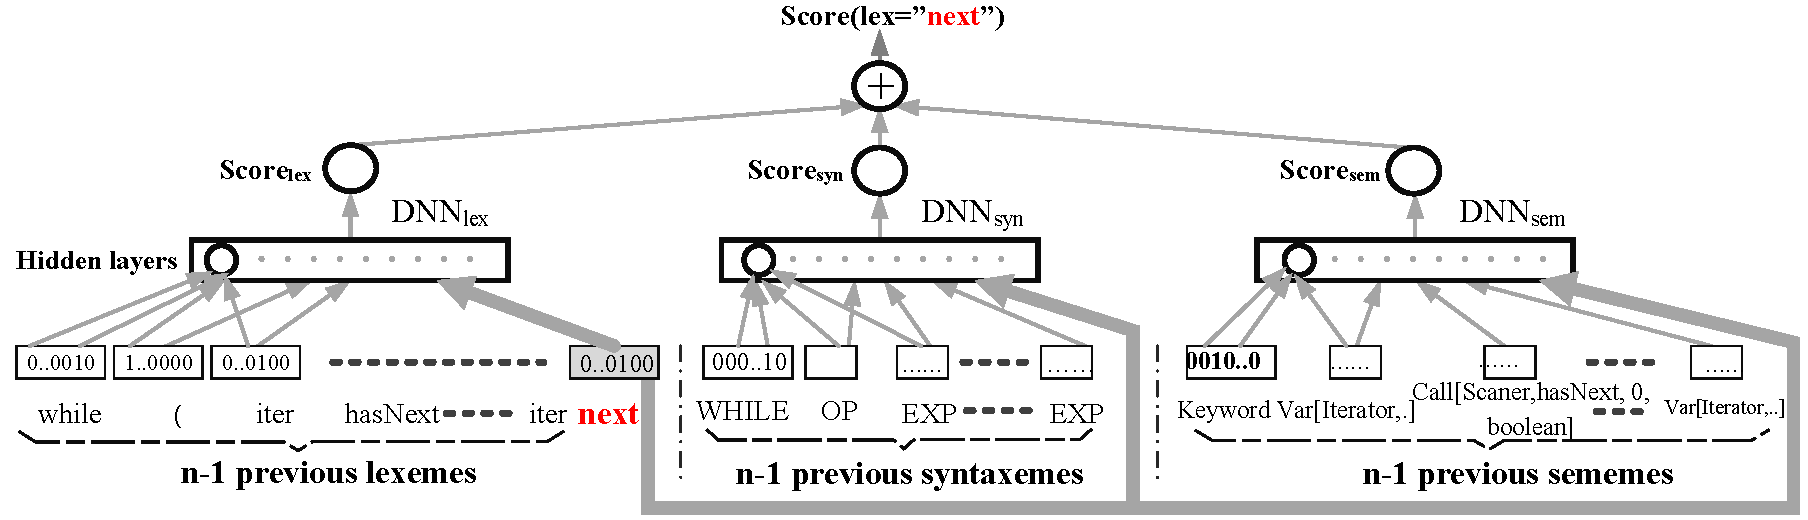
\includegraphics[width=6in]{contextmodel2.pdf} %contextmodel.pdf
\vspace{0.03in}
\caption{Context-aware DNN: Incorporating Syntactic and Type Contexts}
\label{contextfig}
\end{figure*}

\subsection{Overview and Key Ideas}
\label{keyideas}

%To achieve the goal of incorporating syntactic and semantic contexts,
%we design {\tool} with the following key ideas:

%Inspired by the success of DNN, 

We develop {\bf {\tool}}, a DNN-based LM for source
code, that 
%complements the local history of~$n$-gram by additionally
incorporates syntactic and type contexts (Fig.~\ref{contextfig}).
%We adapted Huang {\em et al.}~\cite{huang12}'s model for our new code
%features listed in Section~3:

%1. {\bf Syntaxeme and sememe sequences as contexts}. While the
%traditional DNN LM uses only $n$-1 prior lexical tokens (words),~we
%also attempt to parse the current file and derive the syntaxeme and
%sememe sequences for those tokens (if possible), and use those
%sequences as contexts. We expect that with more precise information on
%the current syntactic unit and on data/token types, DNN LM will be
%able to capture patterns at higher abstraction levels, thus, leading
%to more correct suggestion of the next token. For example,
%in Figure~\ref{contextfig}, with the token \code{hasNext} and the
%sememe \code{CALL [Scanner, hasNext, 0, boolean]} being in the
%contexts, {\tool} could rank the token \code{next} of \code{Scanner}
%higher in the output since \code{hasNext} of a \code{Scanner} object
%is often followed by a call to \code{next}. Instead of using only one
%DNN for the lexemes as in DNN LM, we input each lexeme and its syntax
%and semantic contexts into two additional DNNs
%(Figure~\ref{contextfig}), each of which is dedicated to incorporate
%one type of context.

%----------------------------------------------------------------------


1. {\bf Syntaxeme and sememe sequences as contexts}. While existing
deep learning LMs use only lexical code tokens with limited contexts,
we also attempt to parse the current file and derive the syntaxeme and
sememe sequences for those tokens (if possible), and use those
sequences as contexts. 

%We expect that with information on the current syntactic unit and
%data/token types, {\tool} is able to capture code patterns at higher
%abstraction levels.  For example, in Figure~\ref{contextfig}, with the
%token \code{hasNext} and the sememe \code{CALL [Scanner, hasNext, 0,
%    boolean]} being in the contexts, {\tool} could rank the token
%\code{next} of \code{Scanner} higher since \code{hasNext} of a
%\code{Scanner} object is often followed by a call to \code{next}, thus
%improving accuracy.


2. {\bf Multiple-prototype model (DNNs).} Instead of using only one
DNN for all sequences at three levels, we input each lexeme and its
syntax and type contexts into two additional DNNs, each of which is
dedicated to incorporate one type of context (See Fig.~\ref{contextfig}
for the model).
%
As shown in Huang {\em et al.}~\cite{huang12}, using a single DNN
would not capture well different meanings of the same lexeme (e.g.,
\code{next}) in different contexts (e.g., \code{LinkedList.next} or
\code{Scanner.next()}) as the model is influenced by all of them. They
showed that using multiple DNNs for multiple
representations in different contexts capture well a word in different
usages.
%When word meaning is still ambiguous given local context, we expect
%that information in other contexts can help disambiguation.
%\cite{huang12}.

3. {\bf Training objectives.}  There are following objectives in
training for {\tool}: 1) to train the first DNN to learn to determine
the potential next code token based on the $n$-1 {\em previous
  lexemes}, and 2) to train the two additional DNNs for contexts to
discriminate each correct next token $c$ from other tokens in the
vocabulary {\em given the window of $n$-1 previous lexemes} and {\em
  the syntactic/type contexts of that token $c$}. 
%
That is, the score should be large for the actual~next token, compared
to the score for other tokens.
%
Specifically, let us use $lex$ to denote the current sequence of $n$-1
prior lexemes. We aim to train {\tool} to discriminate the actual next
token $c$ (appearing~after $lex$) from the other tokens in the
vocabulary.
%
Let $Score_{syn}$ and $Score_{sem}$ be the scoring functions for two
DNNs  modeling syntactic and type contexts.  We aim
that with the input $lex$, they give the scores $Score_{syn}(c,syn)$
and $Score_{sem}(c,sem)$ for the correct token $c$ much higher than
the scores $Score_{syn}(c',syn)$ and $Score_{sem}(c',sem)$ for any
other token $c'$ in the vocabulary.
%
$syn$ and $sem$ are the sequences of $n$-1 prior syntaxemes and $n$-1
prior sememes representing the contexts for $c$ and $lex$. In
general, one can use any subsequences of the syntaxeme and sememe
sequences for the tokens from the beginning of a file to $c$ as
contexts.
%
However, performance will be an issue when the sequences are
long. Thus, we~used the same length ($n$-1) for syntaxeme and sememe
sequences.



As an example, we want to have the scores \code{$Score_{syn}$} and
\code{$Score_{sem}$} for the token \code{next} of \code{Scanner} to be
higher than the scores for other tokens. Mathematically, as 
in~\cite{huang12,collobert08}, we use a training objective
$O(c,syn)$ that minimizes the ranking loss for each pair of token $c$
and sequence $syn$ in a file, and gives the margin of 1 between two
such scores. Thus, for the sequence $lex$ ending with $c$, it is computed as in the following formula (1):
\[
O(c,syn) = \sum\limits_{c' \in V} max (0,1 - (Score_{syn}(c,syn) - Score_{syn}(c',syn)))
\]
If the margin between the two scores for $c$ and $c'$ is smaller than
1, the $2^{nd}$ argument in the $max$ function is greater than~0.  If
the margin is greater than 1, the $max$ function returns 0, helping
the objective $O$ reach its minimum.
%
Thus, by using the $max$ function, we aim to minimize that ranking
loss for $(c,syn)$.  The same training objectives $O(c,lex)$ and
$O(c,sem)$ are used for lexeme and sememe sequences.


\subsection{Model Architecture and Details}

\begin{figure}[t]
\centering
\includegraphics[width=3.2in]{msr17-dnn2.pdf} %dnn.pdf 0.47
\vspace{-0.06in}
\caption{Deep Neural Network Language Model for Source Code}
\label{dnnfig}
\end{figure}

Fig.~{\ref{dnnfig}} shows model architecture. It takes as input
3 levels of lexemes, syntaxemes, and sememes to
predict the next lexeme.
%
For training, for each sequence $s$ of length $n$, the correct lexeme
$c$ at the $n^{th}$ position of $s$ is fed into the input $lex_n$,
which is actually fed into three DNNs for three levels
(Fig.~\ref{contextfig}).
% Tien
%For training, the correct lexeme $c$ at the $n^{th}$ position of a
%sequence $s$ of length $n$ is fed into the input $lex_n$, which is fed
%into 3 DNNs at 3 levels as explained in Figure~\ref{contextfig}.
%
Three sequences of length $n$-1 for lexemes, syntaxemes, and sememes
corresponding to $s$ are fed into the other inputs.
%
For predicting, each candidate~$c$ in the lexeme vocabulary is fed
into the input $lex_n$ and $Score(c)$ is computed and normalized
(representing how likely $c$ is the next~token of the input~sequ\-ence
$lex_1, ..., lex_{n-1}$). All candidates are ranked via
their scores. 
%Details on training/predicting are given later.
The projection layer could be used in each DNN.

%lex_n = w_i

%score (lex_n = w_i) / sum (score (w_i))  (i from 1 to |V|)

%\vspace{0.03in}
\noindent {\bf Lexical level.} The input at this level is the
concatenated discrete feature vectors of $n$-1 prior lexemes $lex_1,
..., lex_{n-1}$ of the current $lex_n$.
%
Each lexeme is represented by a vector where only the index of that
lexeme is one.
%(all others are zeros). 
The role of projection for lexemes is for {\em word embedding}, i.e.,
to {\em map each lexeme to a continuous feature space} in the same manner in
Word2Vec~\cite{word2vec} (DNN LM also used projection):
%We expect that the ``related'' lexemes are mapped to nearby locations
%along some dimensions in that space:

${h_1}(y) = \tanh \left( {\sum\limits_{x = 1}^{|V|} {w_p(x,y)i(x)} +
  b_p(y)}\right),\forall y = 1, \cdots ,{M_1}$ 

%M_1=n-1

\noindent $i(x)$ is the value of node $x$ at the input; $h_1(y)$ is
the output value~of node $y$ in this projection layer; $w_p(x,y)$ is
the weight of the connection from input $x$ to output $y$, and
$b_p(y)$ is a bias value for node $y$; $M_1$ is the number of outputs
of this layer; and $V$ is the vocabulary.

%Mathematically, the formula (1) in Section~\ref{dnnbackgroundsec} is
%used but $p(y)$ is replaced by $h_1(y)$ and $M_p=M_1=n$-1. 

%($h_1(i)$ is the mapping from the input). 

Then, the output feature~vectors of this layer for $n$-1 prior lexemes
are concatenated with $lex_n$: $h_1 = [h_1(1);...; h_1(M_1);lex_n]$.
To compute the score of a node $y$ at the lexical level, we have:
\[\begin{array}{l}
{lex}(y) = \tanh \left( {\sum\limits_{x = 1}^{n} {w_{lex}(x,y){h_1}(x)} + b_{lex}(y) }\right),\forall y = 1, \cdots ,{M_{lex}}\\
Score_{lex} = \sum\limits_{y = 1}^{{M_{lex}}} {w'_{lex}(y){lex}(y) + b'_{lex}}  \quad \quad \quad \quad \quad \quad \quad \quad \quad \quad (2)
\end{array}\]
where $w_{lex}$ and $w'_{lex}$ are the weights at the lexical
level. $b_{lex}(y)$ and $b'_{lex}$ are the bias values for node $y$ here.

%\vspace{0.03in}
%\noindent {\bf Syntactic level.} For the score from the syntactic
%context DNN, we use the {\em sequence of $n$-1 syntaxemes} corresponding to
%the prior tokens, i.e., $n$-1 syntaxeme units \code{$syn_1$}, ...,
%\code{$syn_{n-1}$}.

\vspace{0.03in}
\noindent {\bf Syntactic level.} For the score from the DNN for syntactic
context, we use the {\em sequence of $n$-1 prior syntaxemes}
\code{$syn_1$}, ..., \code{$syn_{n-1}$} as context, assuming that $syn_n$ is the
syntaxeme for $lex_n$. A lexeme corresponds to only one syntaxeme, but
a syntaxeme can have multiple lexemes.
%
%Note that this is our design choice \#1. For the second, all
%syntaxemes for the tokens from the beginning of the file to the
%current position $n$ are used.
%
Each syntaxeme is represented by a vector where only the index of that
syntaxeme in the vocabulary is set to 1, while all others are 0s.
To form the syntactic context, we concatenate the vectors of $n$-1
syntaxemes with the vector of the lexical token $lex_n$ right
after the current lexical sequence $lex_1$, $lex_2$, ...,
$lex_{n-1}$. Thus, we have the combined vector $syn_h = [syn_1,
  syn_2,..., syn_{n-1}, lex_n]$. To compute the score for a node $y$
at the syntactic level, we use:
\[\begin{array}{l}
{syn}(y) = \tanh \left( {\sum\limits_{x = 1}^{n} {w_{syn}(x,y){syn_h}(x)} + b_{syn}(y) }\right),\forall y = 1,.,{M_{syn}}\\
Score_{syn} = \sum\limits_{y = 1}^{{M_{syn}}} {w'_{syn}(y){syn}(y) + b'_{syn}} \quad \quad \quad \quad \quad \quad \quad \quad \quad (3)
\end{array}\]
where $w_{syn}$ and $w'_{syn}$ are the weights at the syntactic
level. $b_{syn}(y)$ and $b'_{syn}$ are the bias values for a node $y$.
%at this level.

%here

During training, we will select a subset in the lexical vocabulary and
replace $lex_n$ with each of tokens in that subset to form multiple
combined vectors $syn_h$.
%several combined vectors will be formed by replacing
%$lex_n$ with several other words in the lexical vocabulary. 
The training objective is to minimize $O(lex_n,syn)$, i.e., the
ranking loss for each pair of token $lex_n$ and sequence $syn$
(Section~\ref{keyideas}). Note that, in formula~(1),
$Score_{syn}(c,syn)$ is equal to $Score_{syn}$ in formula~(3) where $c
= lex_n$ and $syn = [syn_1, ..., syn_{n-1}]$.

\vspace{0.03in}
\noindent {\bf Type level.} To compute the score from the DNN for
type context, we perform a similar process as the one at the
syntactic level, except that the syntaxemes are replaced by the
sememes of the current lexical sequence. That is, from the combined
vector for the type context, $sem_h = [sem_1, sem_2,...,
  sem_{n-1}, lex_n]$, we compute $sem(y)$ and $Score_{sem}$ as in
(3). The number of hidden nodes is $M_{sem}$. The weights will be
learned via training.
%
Similarly, the training objective is to minimize the ranking loss
$O(lex_n,sem)$ for each pair of token $lex_n$ and sequence
$sem$.


\vspace{0.02in}
\noindent {\bf Final score.} The~final score for a lexical token is
the normalized score of the sum of three scores over all~tokens.
%possible $w_i$ in~$V$.

%$Score$=$Score_{lex}$+$Score_{syn}$+$Score_{sem}$.

%The~final score for each lexical token $w_i$ is the sum of all of its
%scores at three levels:
%$Score$=$Score_{lex}$+$Score_{syn}$+$Score_{sem}$.
%----

%$Score$ at three levels and used for ranking in prediction.

%The scores are used to rank the tokens for prediction.

%---
%\vspace{0.03in}
%\noindent {\bf Semantic level.} To compute the score from the semantic
%context DNN, we perform a similar process as the one at the syntactic
%level, except that the syntaxemes are replaced by the sememes of the
%current lexical sequence. First, to form the semantic context, we
%concatenate the vectors of $n$-1 sememes with the vector of the next
%lexical token $lex_n$ right after the current lexical sequence. Thus,
%we have the combined vector $sem_h = [sem_1, sem_2,..., sem_{n-1},
%  lex_n]$. To compute the score for semantic context, we use a
%two-layer neural network as follows:
%\[\begin{array}{l}
%{sem}(y) = \tanh \left( {\sum\limits_{x = 1}^{n} {w_{sem}(x,y){sem_h}(x)} + b_{sem}(y) }\right),\forall y = 1, \%cdots ,{M_{sem}}\\
%Score_{sem} = \sum\limits_{x = 1}^{{M_{sem}}} {w'_{sem}(x,y){sem}(x) + b'_{sem}(y)} \quad (4)
%\end{array}\]
%$w_{sem}$ and $w'_{sem}$ are the weights at the semantic
%level. $b_{sem}(y)$ and $b'_{sem}(y)$ are biases at this level.
%Similarly, the training objective is to minimize the ranking loss
%$O(lex_n,sem)$ for sequences.
%------------

%Three output vectors of three input layers corresponding to lexical,
%semantic and syntactic levels will be concatenated and calculated by
%hidden layers of our model. The hidden layers can include many layers
%with different number of computation nodes at each layer. The task of
%each layer is to learn the link between syntactic, semantic and
%lexical at the corresponding abstraction level.

%The output of hidden layer will be used in output layer to estimate
%the probability that a lexical with index i in dictionary will appears
%at location n. The index i with high probability will be used to infer
%the corresponding lexeme at location n.




%The syntactic input layer takes representative vectors of $n-1$
%previous syntactic tokens.  Each syntactic token is the label
%syntactic role of corresponding lexical token. For examaple, syntactic
%tokens corresponding of \code{System . out . println (); } will be
%\code{MethodCall(System, . , out, . , prinln, ( , )), Term(;)}. The
%representative vectors are constructed similarly to those in lexical
%and semantic levels.

%The lexical input layer takes representative vectors of $n-1$ previous
%lexical tokens.  The representative vector of each token includes the
%value of 1 for element at index of the token's label in the
%dictionary. The other element will have value of 0. Hence, if the
%dictionary of all token's label has $V$ words, the representative
%vector will have 1 element of value 1 (at index of the token) and
%$V-1$ elements having value of 0.

%The semantic input layer takes representative vectors of $n-1$
%previous semantic tokens.  Each semantic token is the semantic
%annotation of corresponding lexical token in $n-1$ tokens.  For
%example, semantic annotation of tokens of \code{System . out . println
%  (); } will be \code{Type(System, System), Punc(.),
%  Field(OutputStream, out), Punc(.), MethodCall(void, println),
%  Punc((), Punc())}.  The representative vector of each token is
%constructed similarly to that for lexical token, i.e.  one element at
%dictionary index of the token have value of 1 and the others have
%value of 0.

%At input, our model will treat each level in the similar way. That is,
%the $n-1$ representative vectors of $n-1$ tokens will be concatenate
%with their sequential order. The combined vector (with length of
%$(n-1)V$) will be processed with the input layer $I$. The role of $I$
%is to projects the sparse vectors representing $n-1$ tokens to the
%corresponding vectors in continuous space. That step is important due
%to two reasons discussed in section {\ref{nnlmsec}}.

%\vspace{0.03in}

\subsection{Training and Predicting}

\noindent {\bf Training.}  We parse each file in the training
corpus to create lexeme, syntaxeme, and sememe sequences. We collect
all sequences of lexemes with a fixed length $n$: $[lex_1, lex_2,...,
  lex_n]$. The corresponding syntaxeme $syn_{n-1}$ and sememe
$sem_{n-1}$ of $lex_{n-1}$ are identified. We then collect $n$-1 prior
units of lexemes $lex=[lex_1, lex_2,..., lex_{n-1}]$, syntaxemes
$syn=[syn_1, syn_2,..., syn_{n-1}]$ and sememes $sem=[sem_1,
  sem_2,..., sem_{n-1}]$, and use them as input to {\tool} in
Fig.~\ref{dnnfig}. 

The token $lex_n$ is used as the correct next token and fed into the
input labeled $lex_n$. The score for that token is computed with the
current weights (weights are initialized in the beginning). Then,
{\tool} randomly selects a lexical token $c'$ (different from $lex_n$)
as a negative example for the pair $(lex_n,lex)$, and feeds it into
the input labeled $lex_n$ (instead of using the correct token
$lex_n$). The score $Score(c',lex)$ is computed. The difference of the
scores $Score(lex_n,lex)$ and $Score(c',lex)$ is recorded. Then, the
weights are updated for \code{DNN}$_{lex}$ to minimize the value of
the objective $O(lex_n,lex)$ (Section~\ref{keyideas}) by taking a
gradient step with respect to this choice $c'$. That is, we take the
derivative of the ranking loss with respect to the weights of the DNN.
%as in training for Huang's model~\cite{huang12}. 
{\tool} repeats the process for other token $c''$ in the lexeme
vocabulary until reaching a certain number of iterations. As suggested
in~\cite{huang12}, when there is sufficiently large number of
iterations, the quality is as good as using stochastic gradient
descent. The training process continues in the same way to train the
weights for the two other DNNs for syntaxemes and sememes except that
we use $Score(lex_n,syn)$ and $Score(lex_n,sem)$. Details on objective of minimizing ranking loss can be found
in~\cite{collobert08}.


%the other tokens $c'$ are used in place of $lex_n$ and their scores
%are computed. The weights will be adjusted to minimize the values of
%the objectives $O(lex_n,lex)$, $O(lex_n,syn)$, and $O(lex_n,sem)$ for
%each possible group of ($lex_n$, $lex$, $syn$, $sem$) found in the
%corpus.

%For efficient training, we followed the multi-objective joint training
%process by Collobert {\em et al.}~\cite{collobert08}. The process
%starts with the DNN for lexemes (\code{DNN}$_{lex}$). We randomly
%choose a lexical token $c'$ (differing from $lex_n$) as a negative
%example for each group ($c'$, $lex$, $syn$, $sem$). Then, the weights
%are updated for \code{DNN}$_{lex}$ via backpropagation by taking a
%gradient step with respect to this choice $c'$. That is, we take the
%derivative of the ranking loss with respect to the weights of the
%DNN. Next, the process repeats the same for the DNNs for syntaxemes
%and sememes. As suggested in~\cite{huang12}, we repeat it until reaching
%a certain number of iterations. More details are in~\cite{collobert08,huang12}.

%1. Select the next task.
%2. Select a random training example for this task.
%3. Update the NN for this task by taking a gradient
%step with respect to this example.
%4. Go to 1
%-------------------------

%For training, we follow the standard training procedure for deep
%neural network (DNN)~\cite{dnnbook} except for the pre-processing,
%computing the scores at three levels (see the above formulas), and the
%training objective. For the pre-processing, all the programs in the
%training corpus are processed to produce sequences of lexemes,
%syntaxemes, and sememes.  Each window of size $n$ ($n$-gram) is
%processed. The corresponding $n$-grams of syntaxemes and sememes are
%extracted. The $n$-1 elements of each of the lexeme, syntaxeme, and
%sememe sequences are used as the input for training. The scores for
%tokens are computed including for the last lexical token $c$ in the
%current $n$-gram. We use the ranking-loss training objective as
%in~\cite{collobert08}. That is, we aim to minimize the ranking loss
%$O$ for each sequence in the formula (2) (i.e., where the last token
%$c$ is replaced with others).

\vspace{0.02in}
\noindent {\bf Prediction.} At a point $L$ of suggestion in a program,
we process the code using PPA~\cite{ppa08} to construct the sequences
of syntaxemes and sememes up to $L$. For a fixed value of $n$, we
collect $n$-1 prior lexemes, syntaxemes, and sememes (from the last
token before $L$) and use them as the input of {\tool}. Then, each
token $c$ in the~vocabulary $V$ will be fed into the input labeled
$lex_n$ in Fig.~\ref{dnnfig}.~The score for $c$ is
computed and normalized to rank how likely the next token is $c$.
%All tokens in the lexical vocabulary are ranked based on their scores.



